\section{DeepSmith}

DeepSmith is our open source test-case generator for compiler fuzzing~\footnote{DeepSmith available at: \emph{[URL redacted for double-blind review]}}. Figure~\ref{fig:deeptune} provides an overview of the system. Our compiler test-case generation approach consists of two parts: first, a generative model for code samples inferred from open-source codes; the second, test-case construction.


\subsection{Generative Model for Program Codes}

We extend prior work on synthetic program generation using Long Short-Term Memory (LSTM) networks~\cite{Cummins2017a}. An initial seed corpus of 10k OpenCL kernels is mined from GitHub, using an oracle compiler (LLVM 3.9) to reject files that are not well-formed or do not contain instructions. The corpus is preprocessed using a custom LLVM pass to normalize syntactic choices --- a uniform code style is enforced to ensure consistent use of braces, whitespace, identifier names, etc. The preprocessed corpus is encoded using a hybrid token/character-level encoding~\cite{Cummins2017b}. \cc{More detail\ldots}

LSTM networks model the vocabulary distribution over the encoded corpus. We use a two layer LSTM network of 512 nodes each, trained using Stochastic Gradient Descent for 50 epochs, with an initial learning rate of 0.002 and decaying by a factor of a half every 5 epochs. % We use TensorFlow to implement the LSTM networks, with the entire generative model requiring less than 200 lines of Python, and is not specialized to OpenCL.

The trained network is sampled to generate new programs. The model is seeded with the start of a kernel (\texttt{\_\_kernel void}), and sampled token-by-token. A ``bracket depth'' counter is incremented or decremented upon production of \texttt{\{} or \texttt{\}} tokens respectively, and sampling terminates once the bracket depth reaches zero. The generated sequence of tokens are then concatenated and used as the generated program.


\begin{figure}
  \centering
  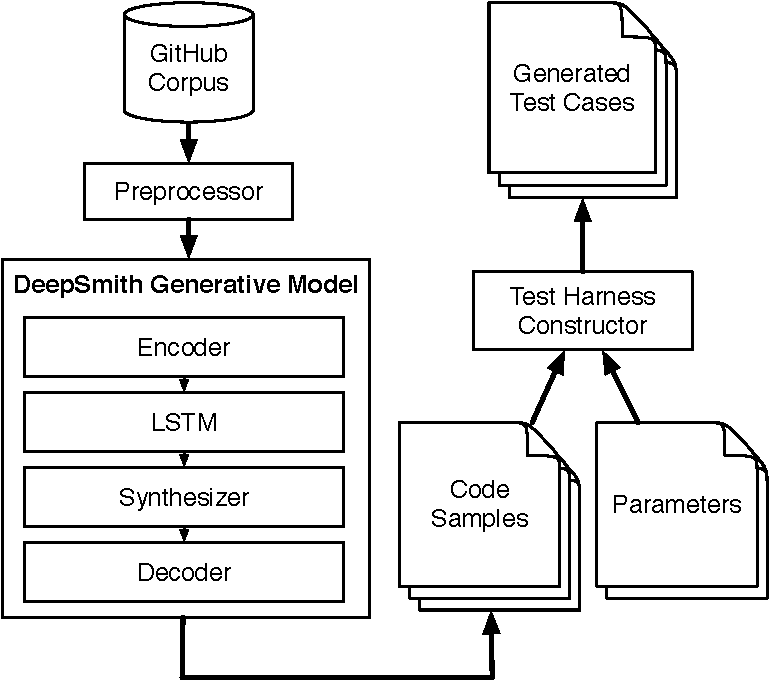
\includegraphics[width=.80\columnwidth]{img/deepsmith} %
  % \vspace{-2em}%
  \caption{%
    Test-case generation. An corpus of programs from GitHub is used to seed a generative model for program code, which are parameterized to construct test-cases.%
  }%
  \label{fig:deeptune}
\end{figure}


\subsection{Test-case Construction}

OpenCL is an embedded compute kernel language, requiring host code to compile, execute, and transfer data between the host and device. For the purpose of compiler fuzzing, this requires a \emph{test harness} to run the generated OpenCL programs.

At first, we used the test harness of CLSmith. CLSmith kernels accept no inputs, and each thread computes the same value which is stored in a \texttt{unsigned long} buffer. The fixed function prototype means that they have a single re-usable test harness which may compile any CLSmith kernel, run it, and prints the output. We found this fixed harness to be too inflexible for our needs. This prototype is not a common OpenCL use case (only 5.6\% of GitHub kernels accept a single argument, of which 3.4\% are \texttt{ulong}, 0.2\% of the total).
% $ grep -E '^__global (.*)\* A$' github-arguments.txt | wc -l     -> 294
% $ grep '^__global ulong\* A$' ~/src/project_b/difftest/github-arguments.txt | wc -l     -> 10
To test a more expressive range of kernels, we created a tool to generate host code capable of driving arbitrary OpenCL kernels, allowing us to create a unique test harness for each generated program.

For a given OpenCL kernel, we first parse the function prototype in order to determine the expected arguments. We then generate host data to feed to these arguments - supporting scalars and arrays of all primitive and vector types. We parameterize data generation with a single value $n$. Input arrays are populated with values {$[1 \ldots n]$}; scalar values are given value $n$. We then enqueue the kernel with $n$ threads. The \emph{output} of a program is the values of all non-const arguments after kernel execution. For each program, we generate two test harnesses, one where $n=1$ (i.e. a single thread computing a single result) and one where $n = 2048$.

Since we do not guarantee that the generative model samples are well-formed, it may not be possible to parse the function signature. In this case, a ``compile-only'' stub is generated, which only compile the kernel, without generating input data or executing the compiled kernel.

We note that, unlike the generative model, this test harness construction is language-specific and the design stems domain knowledge. Still, it is a relatively simple procedure, consisting of a few hundred lines of Python.

% SELECT (SUM(compile_only) / (
% SELECT COUNT(*)
% FROM CLgenResults results
% INNER JOIN CLgenMetas meta ON results.id = meta.id
% WHERE cumtime < 48 * 3600
% )) * 100 as '% compile-only'
% FROM CLgenResults results
% INNER JOIN CLgenMetas meta ON results.id = meta.id
% INNER JOIN CLgenHarnesses harnesses on results.testcase_id = harnesses.id
% WHERE cumtime < 48 * 3600;
% 21.5\% of test-cases are compile-only stubs.


\subsection{Test-case Execution}

\begin{figure}
	\centering %
	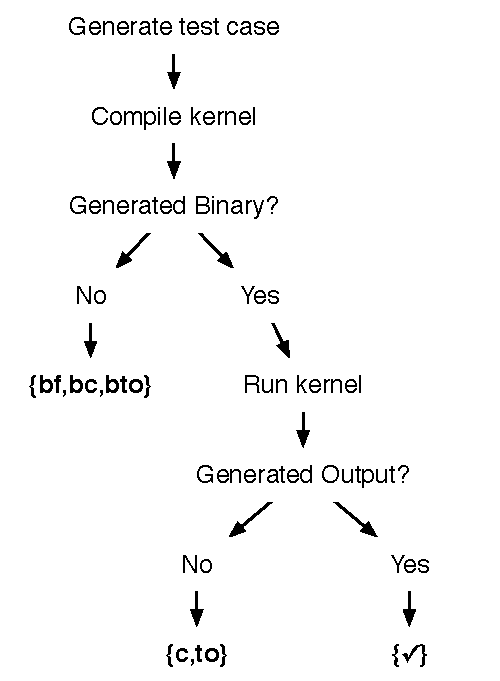
\includegraphics[width=.62\columnwidth]{img/test_process}%
	\caption{%
		Test-case execution, and possible outcomes. Each test-case execution produces one of six possible outcomes: \{bf,bc,bto,c,to,\cmark\}.%
	}%
	\label{fig:test-process} %
\end{figure}

% We classify the result of executing a test-case into one of six classifications: build failure (\textbf{bf}), build crash (\textbf{bc}), runtime crash (\textbf{c}), or pass (\textbf{\cmark}). A \textbf{bf} occurs when compilation of a kernel fails, usually accompanied by an error message. A \textbf{bc} outcome occurs when the compiler crashes. A \textbf{c} outcome occurs when the program crashes during execution. The \textbf{bto} and \textbf{to} outcomes occur when the program compilation or execution time out, respectively.

Executing a test-case on a configuration leads to one of six possible outcomes: \textbf{\{bf,bc,bto,c,to,\cmark\}}, illustrated in Figure~\ref{fig:test-process}.

A \emph{build failure} (\textbf{bf}) occurs when online compilation of the OpenCL kernel fails, usually accompanied by an error diagnostic. A \emph{build crash} (\textbf{bc}) or \emph{build timeout} (\textbf{bto}) outcome occurs if the compiler crashes or fails to produce a binary within 60 seconds, respectively. For compile-only test-cases, a \emph{pass} (\textbf{\cmark}) is achieved if the compiler produces a binary. For test-cases in which the kernel is executed, kernel execution leads to one of three potential outcomes: \emph{runtime crash} (\textbf{c}) if the program crashes, \emph{timeout} (\textbf{to}) if the kernel fails to terminate within 60 seconds, or \emph{pass} (\textbf{\cmark}) if the kernel terminates gracefully and computes an output. 
%
%\begin{enumerate}
%	\item \emph{Build failure} (\textbf{bf}) Online compilation of the OpenCL kernel fails, usually accompanied by an error diagnostic.
%	\item \emph{Build crash} (\textbf{bc}) The compiler crashes during online compilation of the OpenCL kernel.
%	\item \emph{Build timeout} (\textbf{bto}) Online compilation of the OpenCL kernel exceeds the timeout of 60 seconds.
%	\item \emph{Runtime crash} (\textbf{c}) Compilation of the OpenCL kernel succeeds gracefully, but the program crashes during kernel execution.
%	\item \emph{Runtime timeout} (\textbf{to}) Compilation of the OpenCL kernel succeeds gracefully, but program execution exceeds the timeout of 60 second.
%	\item \textbf{\cmark} \emph{Completion} The program terminates gracefully and produces an output.
%\end{enumerate}

When evaluating the outcomes of test-cases, \textbf{\{bc,bto\}} outcomes are of immediate interest, indicative of erroneous compiler behavior. For all other outcomes, \emph{differential tests} are required to expose anomalous behavior.


\subsection{Voting Heuristics for Differential Testing}

Voting is used to expose anomalous outcomes of test-cases. Prior works have formulated random program generation so as to minimize or eradicate the possibility of undefined and unspecified behaviour~\cite{Yang2011c,Le2013a,Le2015}. Recently, work in Skeletal Program Enumeration~\cite{Zhang2017a} has relied on handchecking of C programs and tools such as CompCert~\cite{Leroy2013} and UBsan to detect false-positives. Our approach provides no guarantees of generated program correctness, either with respect to a program being well formed or free from undefined behavior. Instead, we rely extensively on voting across configurations to reveal anomalous outputs.

In prior work, voting on the output of programs across compilers has been used to circumvent the \emph{oracle problem} and determine wrong-code bugs.
% In~\cite{Lidbury2015a}, a configuration is determined to have produced a wrong code result for a kernel if there is a majority output of at least 3 among the \textbf{\cmark} results for the kernel, and the configuration yields a \textbf{\cmark} result that disagrees with the majority.
We extend this approach to describe not only miscompilations, but also anomalous build failures, crashes, and timeouts.

A majority outcome exists if, for for a particular test-case ran on $n$ configurations, at least $\ceil{\frac{2}{3}n}$ configurations produce non-\textbf{\{bc,bto\}} results with the same outcome. We classify anomalous results with respect to the majority outcome for each test-case.

An anomalous output (\textbf{ao}) occurs if, for a given test-case, the majority outcome is a pass \textbf{\cmark}, at least $\ceil{\frac{2}{3}n}$ configurations compute the same result, and a configuration yields a result which differs from this majority result. An \textbf{ao} result is indicative of a \emph{miscompilation}, a particularly hard to detect class of bug in which the compiler silently emits the wrong code. CSmith is designed specifically to target this class of bug. On the other hand, if the result computed by a program depends on undefined or unspecified behavior, then the result is meaningless. Since DeepSmith programs are not guaranteed to be free from undefined behaviors, additional filtering of test-cases is required to prune false-positives, described in section~\ref{subsec:discussions}.

An anomalous build failure (\textbf{abf}) result occurs if, for a given test-case, the majority outcome not \textbf{bf}, and a configuration yields a \textbf{bf} result. Anomalous build failures

permissive
\emph{integer literal is too large}

anomalous runtime crash (\textbf{ac}), and anomalous timeout (\textbf{ato})

If the majority outcome is 

If the majority outcome is a pass \textbf{\cmark}, the outputs are used to determine a majority \emph{output}. Again, a majority \emph{output} exists of $\ceil{\frac{2}{3}m}$ of the $m$ configurations with \cmark outcomes compute the same result. Any configuration which yields a \cmark outcome whose output differs from the majority is considered a candidate for miscompilation.

% Only 2.3\% of CLSmith programs with anomalous outputs are insensitive to optimization level.

%
%\begin{enumerate}
%	\item \textbf{w} \emph{Wrong code} Program terminates gracefully, but computes a result which differs from the majority output. For a DeepSmith result to be classified with \emph{wrong-code}, we require first that the program passes verification using GPUVerify~\cite{Betts2012}, and that a reference run with Oclgrind~\cite{Price2015} produces no warnings. \cc{Vote on compiler warnings, and optimization sensitivity. This means we way miss bugs which optimization level insensitive, though our experiences testing with CLSmith revealed only discovered 2 such cases}.
%	\item \textbf{bf} \emph{Build failure} Online compilation of OpenCL program fails, whereas the majority of configurations produce a binary. \cc{TODO: with voting to exclude programs which rely on OpenCL 2.0 / compiler specific features}
%	\item \textbf{c} \emph{Runtime crash} One or more OpenCL API calls return an error status during the program execution, or the program crashes.
%	\item \textbf{to} \emph{Runtime timeout} Program execution exceeds the timeout of 60 second, whereas the majority of configurations produce an output.
%\end{enumerate}


\subsection{Discussions}\label{subsec:discussions}

\paragraph{Undefined Behaviors} OpenCL doesn't have the rich tooling of C --- no CompCert and UBSan. GPUverify~\cite{Betts2012} and Oclgrind can catch some errors, but as we have shown in Section~\ref{sec:motivation}, this tool is not without flaws. Compiler warnings are useful for obvious missteps, but our approach still requires some manual inspection. There is much work to be done. We demand that the behavior of test-cases is \emph{portable} and \emph{reproducible}. In some respects this simplifies the execution process.

\paragraph{Floating Points} The OpenCL specifications permit acceptable error bounds (ULP) for floating point operations and builtin functions. Some operations like addition, subtraction, and multiplication are precise; divide permits a small error, and builtins vary widely. Thus two implementation may give different answers that both fit within the allowed ranges (and because errors propagate through operations it's hard to even describe the ULP on the final output). \texttt{half\_} functions permit large error bounds. \texttt{native\_} functions have ``implementation defined'' error bounds. TODO: Denormal numbers may optionally be pushed to zero.

At the moment, we simply rely upon \texttt{printf()} rounding.

\cc{If we difftest across floats:}
CSmith, and by extension, CLSmith, do not support floating point operations. In our observations with testing using CLSmith (described in Section~\ref{sec:vs_clsmith}), we observed that in cases of wrong-code bugs, the computed values are usually entirely incorrect, not only marginally different. We hypothesized that by allowing relaxed comparisons between floating point values, we could still differential test. We permit a margin of deviation for floating point comparisons. This means that if a compiler were to emit wrong code which changes the computed value only subtly, we may miss it; though we have no reason to suggest that such a case is any more likely than a wrong code bug leading the compiler to produce exactly the same output, which neither we or any prior work have noted.

\cc{If we ignore floats:}
Given that not all vendors provide bounds for floating point imprecision, we excluded kernels containing floating points from the wrong-code check. Given knowledge about hardware imprecision, it would be possible to compute threshold for floating point difftests.
% Section 7.4 of OpenCL 1.2 spec.

\paragraph{OpenCL Versions and Extensions} double-point precision in OpenCL 1.2 requires an extension. OpenCL 2.0 extends APIs. Compiler warnings were sufficient to prune these.

\paragraph{Implementation} The generative model itself is language-agnostic and requires less than 200 lines of Python --- a small fraction of that of grammar-based approaches, even excluding the static analysis.